\documentclass[a4paper, 11pt]{scrartcl}

\usepackage{graphicx}
\usepackage[american]{babel}
\usepackage{emoji}
\usepackage{svg}
\usepackage{lipsum}
\usepackage{tikz}
\usepackage{todonotes}
\usepackage{caption}
\usepackage{subcaption}
\usepackage[margin=2cm]{geometry}
\usepackage{float}

\usetikzlibrary{calc, positioning, shapes}

\pagenumbering{gobble}

\newcommand{\backendcolor}{blue!40}
\newcommand{\frontendcolor}{red!40}
\newcommand{\eventcolor}{orange!40}

\newcommand{\technicaldebt}[1]{\tikz[baseline=-0.7ex]\node[scale=0.4, fill=#1, draw, circle, minimum width=1cm] () {};}
\newcommand{\technicaldebtfrontend}{\technicaldebt{\frontendcolor}}
\newcommand{\technicaldebtbackend}{\technicaldebt{\backendcolor}}

\newcommand{\feature}[1][]{Feature#1 \emoji{clipboard}}
\newcommand{\bug}[1][]{Bug#1 \emoji{beetle}}
\newcommand{\event}[1][]{Event#1 \emoji{calendar}}

\newcommand{\storypoint}{\emoji{teddy-bear}}

\newcommand{\personaharald}{Harald \emoji{old-man-medium-skin-tone}}
\newcommand{\personamathilde}{Mathilde \emoji{woman-dark-skin-tone}}
\newcommand{\personasabine}{Sabine \emoji{woman-medium-skin-tone}}
\newcommand{\personamark}{Mark \emoji{man-medium-skin-tone-curly-hair}}

\begin{document}

\setemojifont{TwemojiMozilla}

\section*{Background}

Welcome to MagicSoftware Inc. We are delighted that you are joining us as a new employee today. As you know, we build software for the digitalization of reporting. A year ago, we introduced \glqq agile\grqq\ as our working mode. You will certainly get used to it quickly. Perhaps now it is best to meet your team:

\noindent\personaharald\ is your team lead. He used to be a developer here before he took over the management role. Accordingly, he get give you a helping hand when needed.\\
\personamathilde\ is part of the quality assurance and your contact regarding everything to do with testing.\\
\personasabine\ is the customer manager. That means you don't have to deal with customers yourself. She has your back. At the same time, however, we have a shortage of staff, so Sabine has to help out elsewhere. Please be patient with her.\\
\personamark\ is the customer. You won't be in direct contact with him, but it's good to know who you're actually working for.

\noindent The project will be completed in nine iterations. Some things have been completed by your predecessors. Others have been left undone. But we are sure you will manage. Good luck!

\section*{Game Elements}

\begin{itemize}
    \item 9 event cards
    \item 39 ticket cards, including:
    \begin{itemize}
        \item 27 features
        \item 12 bugs
    \end{itemize}
    \item 12 double-sided tokens for technical debt
    \item 20 bears as tokens for story points
    \item 1 game board
\end{itemize}

\subsection*{Event Cards}

\begin{figure}[H]
    \centering
    \begin{tikzpicture}
        \node[draw, inner sep=0cm, line width = 1mm] (card) {\includegraphics[width=0.3\textwidth]{images/event}};

        \node[anchor=north west, text width = 6cm] (title) at ($(card.north east) + (1cm, -0.3cm)$) {\textbf{Card type}: Events are unforeseen incidents that occur during the project. You will find out whether they have a positive or negative effect during execution.};
        \draw[->, line width = 1mm, dotted] ($(title.north west) + (0mm, -2.5mm)$) -- ($(title.north west) + (-25mm, -2.5mm)$);

        \node[anchor=west, text width = 6cm] (iteration) at ($(card.east) + (1cm, -0.45cm)$) {\textbf{Upcoming Iteration}. There are nine iterations in total.};
        \draw[->, line width = 1mm, dotted] ($(iteration.north west) + (0mm, -2.5mm)$) -- ($(iteration.north west) + (-15mm, -2.5mm)$);

        \node[anchor=south west, text width = 6cm] (foreshadowing) at ($(card.south east) + (1cm, -0.5cm)$) {\textbf{Title}: Hint of what to expect from the iteration.};
        \draw[->, line width = 1mm, dotted] ($(foreshadowing.north west) + (0mm, -2.5mm)$) -- ($(foreshadowing.north west) + (-15mm, -2.5mm)$);
    \end{tikzpicture}
\end{figure}

\subsection*{Tickets}

\begin{figure}[H]
    \begin{tikzpicture}
        \node[draw, inner sep=0cm, line width = 1mm, anchor=west] (bug) {\includegraphics[width=0.3\textwidth]{images/bug}};

        \node[anchor = south, text width = 100mm] (kartenart) at ($(bug.north) + (0mm, 10mm)$) {\textbf{Card Type}: Shows whether it is a feature or a bug. The difference between the two is that only features earn you points, but they also generate technical debt. Bugs do not.};
        \draw[->, line width = 1mm, dotted] (kartenart.south) -- ($(kartenart.south) + (0mm, -13mm)$);

        \node[anchor = north west, text width = 50mm] (startmarker) at ($(bug.north east) + (10mm, -2.5mm)$) {\textbf{Start marker (optional)}: Shows whether the ticket is on the game board at the beginning of the game.};
        \draw[->, line width = 1mm, dotted] ($(startmarker.west) + (0mm, -3.5mm)$) -- ($(startmarker.west) + (-18mm, -3.5mm)$);

        \node[anchor = west, text width = 50mm] (cost) at ($(bug.east) + (10mm, -5mm)$) {\textbf{Cost}: Amount of story points you have to use for the ticket. The fixed cost are the amount of bears on the left side. Additionally, you have to use one storypoint for each technical debt in the corresponding system part.};
        \draw[->, line width = 1mm, dotted] ($(cost.west) + (0mm, 6mm)$) -- ($(cost.west) + (-13mm, 6mm)$);

        \node[anchor = south west, text width = 50mm] (title) at ($(bug.south east) + (10mm, 0mm)$) {\textbf{Title}: A description of the ticket.};
        \draw[->, line width = 1mm, dotted] ($(title.north west) + (0mm, -2.5mm)$) -- ($(title.north west) + (-15mm, -2.5mm)$);

        \node[anchor = north east, text width = 50mm] (system) at ($(bug.north west) + (-10mm, -7mm)$) {\textbf{System part}: Indicates whether the ticket belongs to the frontend or backend.};
        \draw[->, line width = 1mm, dotted] (system.east) -- ($(system.east) + (13mm, 0mm)$);

        \node[anchor = south east, text width = 50mm] (hint) at ($(bug.south west) + (-10mm, 5mm)$) {\textbf{Effect hint}: When processing a ticket, you execute the effect on the back. The effect hint shows whether you have to expect a positive (\tikz[baseline=-1ex]\node[scale=0.4, single arrow, draw, fill=white, rotate=90, minimum height = 1cm, minimum width = 1cm] {};), negative (\tikz[baseline=-0.5ex]\node[scale=0.4, single arrow, draw, fill=white, rotate=270, minimum width = 1cm, minimum height = 1cm] {};) or random (?) effect.};
        \draw[->, line width = 1mm, dotted] (hint.east) -- ($(hint.east) + (27mm, 0mm)$);
    \end{tikzpicture}
\end{figure}

\subsection*{Technical Debt}

Technical debt makes it harder to add more functionality. How much technical debt you have is shown by the corresponding tokens. Frontend debt looks like this: \technicaldebtfrontend. Backend debt like this: \technicaldebtbackend. The physical tokens are these double-sided markers:

\begin{figure}[H]
    \centering
    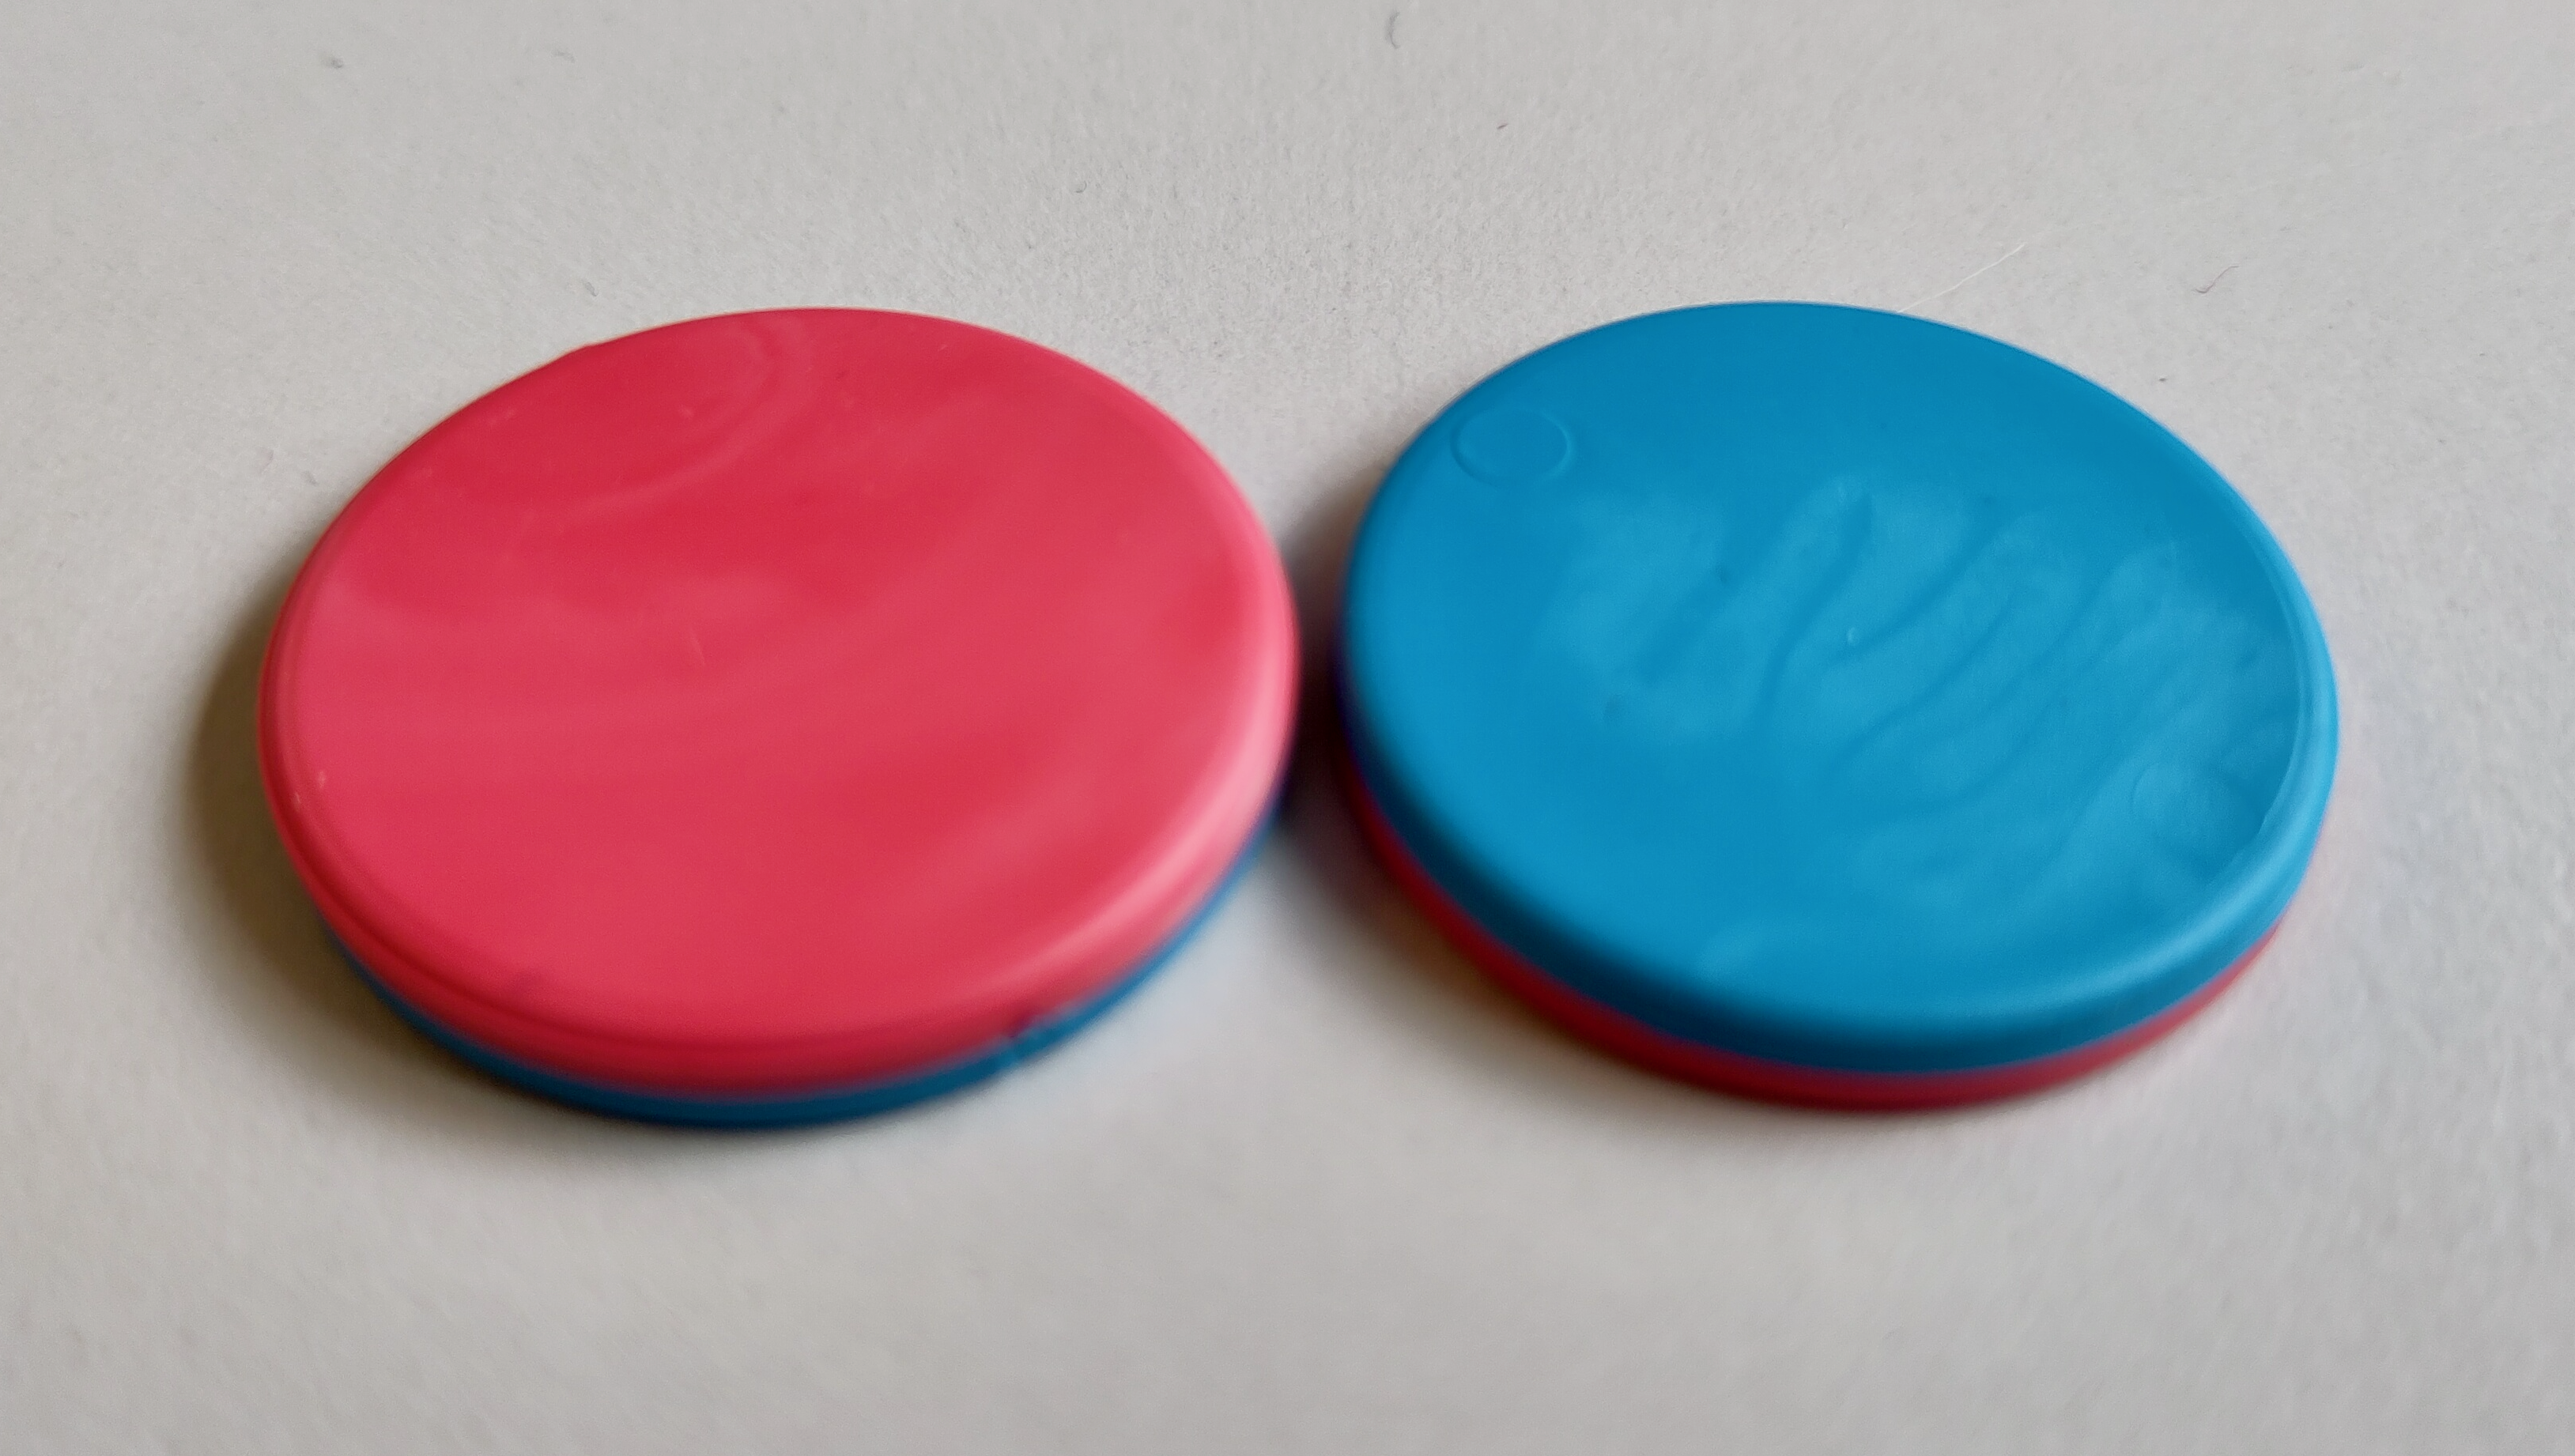
\includegraphics[width=0.3\textwidth]{images/wendechips.png}
\end{figure}

\subsection*{Story points}

Storypoints are a unit of measurement for the effort you have to put into processing a ticket. They are displayed in the text with the following symbol: \storypoint. You have a certain quota of storypoints available per sprint. They regenerate at the end of the sprint. The amount of storypoints available can change due to effects. The physical tokens are these bears:

\begin{figure}[H]
    \centering
    \includegraphics[width=0.25\textwidth]{images/storypoints.png}
\end{figure}

\section*{Setup}

\noindent We have already set the game up. The instructions for that are below. Please check that everything corresponds to the instructions. If anything is different, please let us know.

\begin{itemize}
    \item Sort the events according to iteration. The top card is for iteration 1, the bottom card is for iteration 9. Place them on the event stack.
    \item Pick out the three features with start markers and place them in the backlog.
    \item Shuffle the remaining features and place them on the feature stack.
    \item Pick out the one bug with a start marker and place it in the backlog.
    \item Shuffle the remaining bugs and place them on the bug stack
    \item Place the 13 technical debt tokens next to the board.
    \item Place six story points in the story point field. This is your permanent quota until further notice.
    \item Place the remaining 14 story points next to the playing field.
\end{itemize}

\begin{figure}[H]
    \centering
    \includegraphics[width=\textwidth]{images/spielfeld_aufgebaut.jpg}
\end{figure}

\newpage

\section*{Gameplay}

The game consists of successive rounds or iterations. An iteration consists of the following steps:

\begin{enumerate}
    \item \textbf{Event}: Draw the top card from the event stack and execute its effect.
    \item \textbf{New feature}: Draw the top card from the feature stack and place it into the backlog with the cost calculation facing up.
    \item \textbf{Planning the iteration}: Choose one or multiple actions for the iteration. The possible actions are:
    \begin{itemize}
        \item \textbf{Choosing tickets}: Select one or multiple tickets from the backlog for processing. Put the needed amount of story points on the corresponding ticket. The amount of needed story points is the sum of the fixed price on the left side of the equation and the amount of technical debt in the ticket's system part. \underline{Caution}: If you want to refactor the frontend or backend in this iteration, you cannot select tickets from that system part.
        \item \textbf{Reduction of technical debt / refactoring}: For each technical debt you want to remove by refactoring, you need to use one storypoint. Put the story point on the technical debt to remove. \underline{Caution}: If you refactor in the frontend, you cannot process frontend tickets. The same applies to the backend. You can refactor the frontend and backend at the same time but then you cannot process any tickets.
        \item \textbf{Drawing additionsl feature(s)}: Draw one or more features from the feature stack and put them in the backlog with the cost calculation facing up. This costs one story point for each additional feature.
    \end{itemize}
    \item \textbf{Executing the iteration}: Process everything you planned for the iteration:
    \begin{itemize}
        \item Remove technical debt marked for refactoring
        \item Process the selected tickets by taking one ticket at a time, turning it around and executing its effect. The order in which you process the tickets is up to you.
    \end{itemize}
    \item \textbf{Increasing technical debt}: If you processed at least one feature in the frontend, add exactly one frontend technical debt. Multiple frontend features do not result in multiple fronend debt. The same applies to the backend. Processing bugs does not lead to an increase of technical debt.
    \item \textbf{Checking the end condition}: Check whether one of the end conditions is met. If so, the game ends. Otherwise, prepare the next iteration.
    \item \textbf{Preparing the next iteration}: Put the storypoints used in the planning phase back into the story point field. \underline{Caution}: The amount of available story points can be altered by effects. Sometimes you will have more or less story points available for the next sprint. The effects make clear what to do in that regard.
\end{enumerate}

\section*{End of game and points}

The game ends in one of two ways:

\begin{enumerate}
    \item At the end of an iteration there are nine or more tickets in the backlog. You lose.
    \item You complete all nine iteration without losing. You win.
\end{enumerate}

\noindent If you lost the game, you have 0 points. If you won, each processed feature gives one points. Fixed bugs do not grant points.

\end{document}
